\chapter{The CMS Experiment at the CERN LHC}

The Large Hadron Collider (LHC) at the European Organization for Nuclear Research (CERN)
is the world's largest and most powerful particle collider~\cite{Evans:2008zzb}. It collides protons 
at a center of mass energy of $13\TeV$, and lead ions at $2.76\TeV$ per nucleon.
The protons or ions are brought to collision at the center of four large detectors,
themselves a combination of many detector technologies. 
The particle detectors at the LHC were conceived, developed, and constructed over decades
by collaborations of thousands of scientists from hundreds of nations to
achieve a broad program of research. The detectors were designed and are operated
by mutually exclusive collaborations of researchers working independently,
which enables cross-validation of results while fostering productive competition.

The detector sites along the LHC tunnel are:

\begin{itemize}
  \item A Large Ion Collider Experiment (ALICE) detector~\cite{Aamodt:2008zz}, located at access point 2.
  Designed for the study of lead-ion collisions, especially for the characterization
    of quark gluon plasmas formed in collisions.
  \item A Large Toroidal LHC ApparatuS (ATLAS) detector~\cite{Aad:2008zzm}, located at access point 1.
  A general-purpose detector designed for sensitivity to new physics at the electroweak scale
  decaying to stable SM particles, in particular the 
    discovery and characterization of the SM Higgs boson.
  \item The Compact Muon Solenoid (CMS) detector~\cite{Chatrchyan:2008aa}, located at access point 5.
    A general purpose detector with comparable measurement potential to the ATLAS detector.
  \item The Large Hadron Collider Beauty (LHCb) detector~\cite{Alves:2008zz}, located at access point 8.
  Designed to characterize the production and decay of b-quark hadrons. Particularly
    focused on charge--parity violations in these decays.
\end{itemize}

Results in this thesis are based on an analysis of proton--proton collisions at the LHC 
collected by the CMS detector in 2016. This chapter describes the design principles of the 
LHC and the CMS detector, as well as their operating characteristics in 2016.
  
\section{The Large Hadron Collider}
The principle design considerations of a particle collider are the energy
of the particle collisions, the rate of collisions, and the objects collided.
The collided objects determine the possible interactions which can be probed,
whereas the energy of the collision drives the mass range which can be probed,
subject to the constraint that the produced particle mass $m$ be less than the 
center of mass energy of the collision. As particle interactions are quantum mechanical 
and fundamentally stochastic in nature, the rate of collisions is also 
critical for achieving statistically significant measurements.

Several characteristics of proton--proton (\pp) collisions motivated the decision 
to use protons in the world's highest-energy collisions. Accelerating and
directing particles to collision relies on electric and magnetic forces,
so the collided particles must be electrically charged. 
The only charged, stable, unbound, and fundamental particle is the electron.
Electron--positron collisions have played a major role in the field 
of particle physics, however, because accelerated charged objects
loose energy proportional to $m^{-4}$ via synchrotron radiation,
accelerating electrons to the TeV scale would require a prohibitively large tunnel
to limit the bending force of the accelerator.
Because the mass of the proton is nearly two thousand times greater than the 
electron mass, synchrotron radiation is much less severe for accelerated protons.
However, the proton is a composite object, so the conditions of its constituent
quarks and gluons cannot be directly controlled when
directing the protons to interaction, rather, they must be inferred from 
the properties of the colliding protons. These unknowns, governed by the 
complex structure of the proton, make proton--proton collisions inherently
messier than collisions of fundamental particles. However, the compositeness
of the proton is advantageous due to the rich phenomenology of interactions
proceeding via quarks and gluons. 
Additionally, quark-antiquark pairs are accessible in the proton at high energy
scales, so interactions proceeding via particle--antiparticle annihilation
are still accessible in high energy \pp interactions. Without the need 
to produce antiparticles before bringing them to collision, which was necessary
at lower-energy accelerators---notably the Large Electron Positron Collider (LEP) collider
at CERN and the Tevatron collider at Fermilab in the United States---the LHC is
able to deliver significantly higher interaction rate to complement its high
collision energy.

The LHC was proposed to the CERN council, the management group of the 
laboratory, in 1994, and accepted
with a preliminary budget in 1995. Construction was initially completed in
2008, with full operation beginning in 2009 after setbacks 
encountered in the initial commissioning.
The collider is located on the outskirts
of Geneva, Switzerland and in the nearby French countryside,
which has been the site of the CERN laboratory since it was founded in 1954.
The project was funded by the 20 member states of CERN, as well
as monetary and research contributions from many other nations participating 
in the project, including the United States.

The LHC is situated in a 26.7\unit{km} circumference tunnel, 45--170\unit{m}
below the Swiss and French country side. The tunnel pre-dates the LHC,
having been originally built for the Large Electron Positron (LEP) collider.
It consists of 8 straight sections $528\unit{m}$ in length, and 8 arced sections.
The cross section of the majority of the tunnel is $3.7\unit{m}$ in diameter, with larger excavated
areas at the four experimental caverns and other access points.
The primary motivation for an underground tunnel is to circumvent the high
cost of land acquisition, but underground operation is also advantageous for
reducing the cosmic radiation reaching the experimental cavern and  
for shielding the radiation produced by the LHC. Protons are directed through pipes inside the tunnel, which are held
at high vacuum. The positions and accelerations of the protons are controlled 
by magnetic and electric fields maintained by instrumentation surrounding the 
vacuum pipes. The arced sections are equipped with dipole magnets,
which direct charged objects along a circular path.
The size of the LEP tunnel prohibited the installation of two independent beam
systems, which led to the adoption of a unique "two-in-one" superconducting
magnet design~\cite{temp}, shown in Fig.~\ref{fig:dipoleXsec}. 

\begin{figure}[htbp]
  \centering
   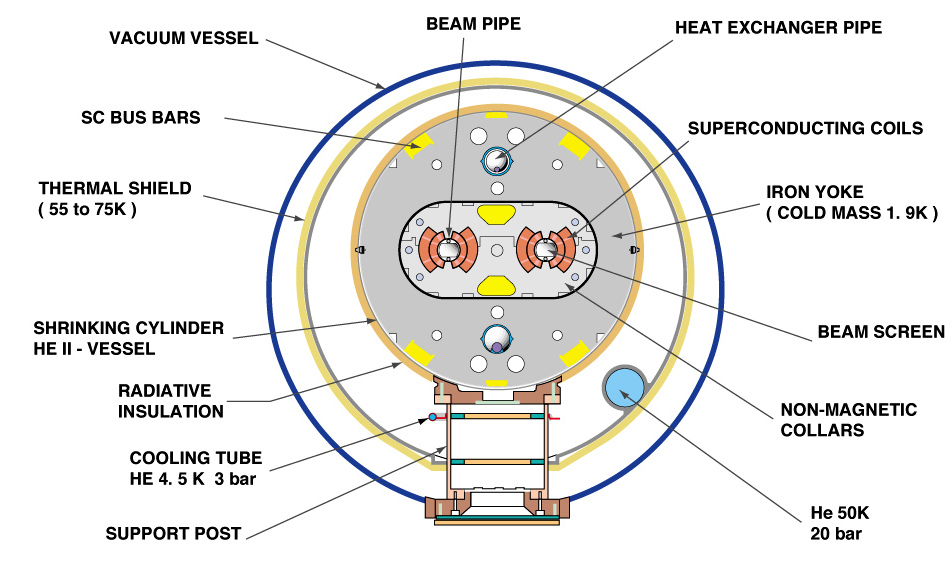
\includegraphics[width=\textwidth]{figures/LHCandCMS/dipoleXSec.jpeg}
  \caption{
    Cross section of an LHC dipole magnet~\cite{Jean-Luc:841539}.
        }
 \label{fig:dipoleXsec}
\end{figure}

Neglecting synchrotron radiation,
the primary limitations on the energy of a synchrotron come
from the magnetic field of the bending magnets and the radius of curvature
of the tunnel. For an particle of charge $q$ with velocity $v$ accelerated at
in a circular 
trajectory of radius $R$ trough a magnetic field of strength $B$
The energy $E$ of the particle is given by

\begin{equation}
  E = qBRv \approx qBRc \,,
\label{eq:beamEnergy}
\end{equation}

where $v \approx c$, the speed of light, for $p \gg m$. Increasing the radius
requires a larger tunnel, which is limited by the cost of construction. 
The LHC tunnel size was set by the existing LEP tunnel, so achieving
a sufficient magnetic field was a major focus of the LHC development. 

Dipole magnets with a maximum field strength of $8.33\unit{T}$ were achieved
at an affordable cost through major technological advances. Such a high 
field necessitates the use of superconducting magnets. The magnets 
are constructed of niobium-titanium, and are operated at $1.9\unit{K}$,
lower than any previous accelerator. 
at 
first accelerator to operate 
In particular,
the LHC is the first accelerator to operate 
Because about 80\% of the arced sectors of the LHC are equipped with dipole magnets,
the bending radius of the dipoles is $2.804\unit{km}$, yielding the design energy
of $7\TeV$ per beam from Equation~\ref{eq:beamEnergy}.

Also brief mention of the 

How it accelerates protons (e.g., the system of accelerators)

The magnet design and characteristics 

The RF and bunch characteristics

Focusing beams to collisions


\section{Operation of the LHC in 2016}

\begin{equation}
  \mathcal{L} = \frac{n_b N_b^2 f_\textit{rev}}{A_\text{eff}}
  \label{eq:lumi}
\end{equation}

\section{The Compact Muon Solenoid experiment}

The CMS detector is a general-purpose detector designed to 
study particle production and interactions at the TeV scale.
A major design principle of the CMS detector was the ability to 
probe the nature of electroweak symmetry breaking, which has been
achieved through the discovery and characterisation of a scalar boson
consistent with the SM Higgs boson~\cite{Chatrchyan:2012xdj,Chatrchyan:2013lba}. 
The design of the CMS detector
ensured sensitivity to a Higgs boson with mass up to
$1\TeV$ in its SM decays, as well as sensitivity to a broad class
of BSM theories. In terms of detector performance, these design principles,
as defined in Ref.~\cite{Chatrchyan:2008aa}, are:

\begin{itemize}
  \item Accurate mmuon identification and high momentum resolution, including
    dimuon mass resolution of $\approx 1\%$ at $m_{\mu\mu} = 100\GeV$ and correct charge
    assignment up to $\pt^{\mu}\approx 1\TeV$.
  \item Identification of objects with a short but significantly decay time,
    including tau leptons and b hadrons, which requires fine position resolution 
    close to the interaction point to distinguish their displaced tracks.
  \item Good electromagnetic energy and momentum resolution, achieving
    diphoton and dielectron mass resolution of $\approx 1\%$ at $m_{ee} = 100\GeV$,
    and sufficient granularity to distinguish prompt diphotons from $\pi^{0}$ decays to photons.
  \item Sufficient calorimeter resolution and hermeticity for precise dijet mass
    and missing transverse momentum reconstruction.
\end{itemize}

The CMS detector has a cylindrical geometry. As shown in Fig.~\ref{fig:CMScutaway},
it is built from the combination
of several detector technologies which work in harmony to achieve the outlined design
goals. The following sections briefly describe each of the detector subsystems
which comprise the CMS detector. 
Chapter~\ref{ch:reconstruction} details the ways in which these subsystems 
are used together to reconstruct the physics objects used for the results
presented in this thesis.

\begin{figure}[htbp]
  \centering
   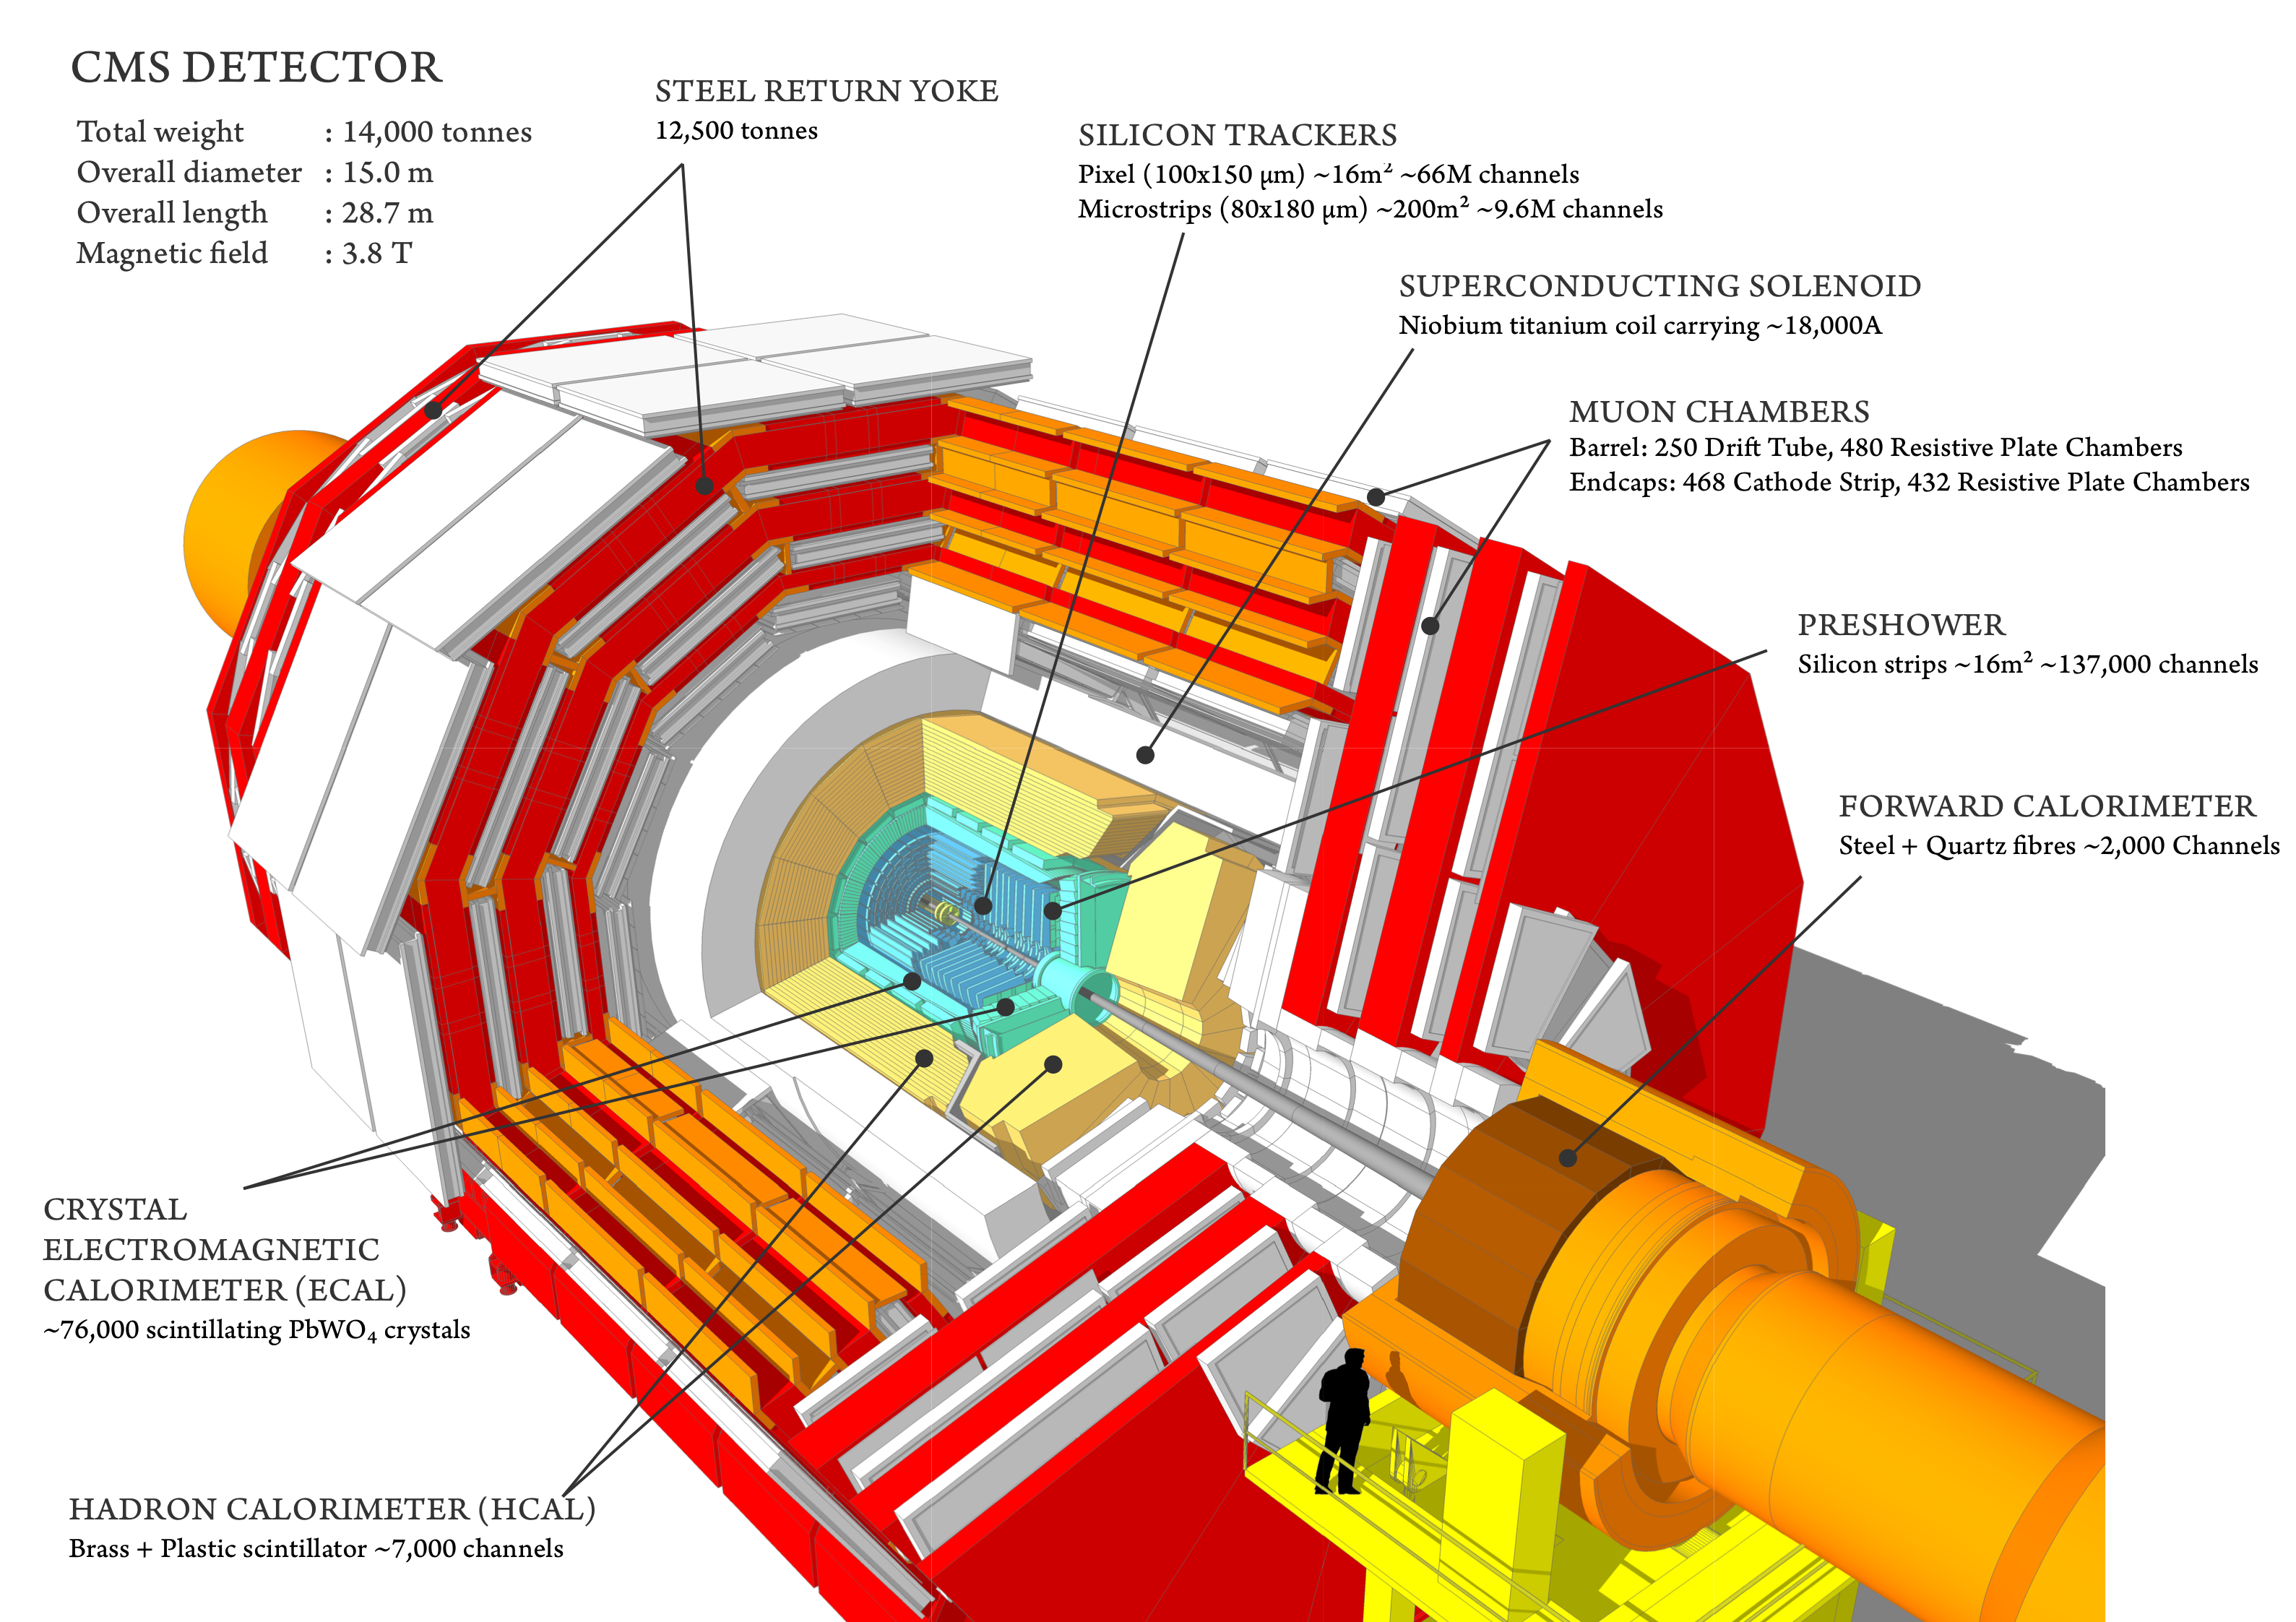
\includegraphics[width=\textwidth]{figures/LHCandCMS/CMScutaway.png}
  \caption{
    A cutaway view of the CMS detector, showing each detector 
    subsystem~\cite{1742-6596-513-2-022032}.
        }
 \label{fig:CMScutaway}
\end{figure}

The coordinate system adopted by CMS, and used in this thesis,
is a right-handed coordinate system with the point $(x, y, z) = (0, 0, 0)$
centered in the detector, at the nominal collision point. The $y$-axis 
is perpendicular to the earth, where vertically upward defines the $+y$ direction.
The $x$-axis is in the plane of the LHC, with the $+x$ direction pointing towards
the center of the ring. The $z$-axis points through the center of the detector
along the direction of travel of the colliding protons, where $+z$ is defined
by the right-handedness of the coordinate system. In polar coordinates, 
the azimuthal angle $\phi$ is measured from the $x$-axis in the $x$-$y$
plane, and the polar angle $\theta$ is measured from the $z$-axis. The radial
coordinate $r$ is defined as $r = \sqrt{x^2 + y^2 + z^2}$.
Because the production of 
particles is preferentially in the forward direction (along
the $z$-axis), it is convenient to introduce the pseduorapidity $\eta = - \ln(\tan{\theta/2})$
for the polar coordinate. The momentum in the transverse direction,
defined as $\pt = \sqrt{p_{x}^2 + p_{y}^2}$, is a particularly important quantity.
because the initial transverse momentum of the collision is zero.
In this thesis, the four-momentum of an object will commonly be expressed as
$p = p(m, \vec{p}) = p(m, \pt, \eta, \phi)$.

\section{The CMS solenoidal magnet}

The central feature of the CMS apparatus is a superconducting solenoid 
of $6\unit{m}$ internal diameter and $12.5\unit{m}$ in length,
constructed from 4 layers of reinforced niobium titanium.
It provides a nearly constant $3.8\unit{T}$ magnetic field inside the solenoidal volume.
The magnetic flux of the solenoid is returned through
a $12 000$-tonne steel yoke, comprising 5 wheels and 2 endcaps,
which is fully saturated to approximately $2\unit{T}$. 
The tracker and calorimeters are situated inside the solenoid, while 
the muon detectors are embedded in the steel return yoke, as shown
in Fig.~\ref{fig:CMScutaway}.

During operation, the CMS solenoid stores approximately $2.4\unit{GJ}$ of 
energy, the largest magnet in the world by this metric. This immense
size leads to a powerful bending radius for charged objects within the detector,
which is a critical metric for particle reconstruction and identification.
In particular, objects of charge $q$ moving
in a magnetic field $\vec{B}$ at velocity $\vec{v}$ experience a Lorentz force,

\begin{equation}
  \vec{F} = q\vec{B} \times \vec{v} \,.
\end{equation}

Because the solenoidal field is constant and aligned along the $z$-direction, 
$\vec{B} = B\hat{z}$, the force is purely in the transverse direction.
Consequently, charged particles within the CMS
solenoid travel along a nearly helical path of radius $R=\pt/\abs{q}B$, where 
small deviations from this path arise from non-uniformity of the field
and interactions in the detector material. The sign of a 
$\pt$ of a particle of known charge can therefore be deduced by measuring its radius of
curvature. The bending power of the magnet $BR$ is therefore a critical 
parameter determining the detector capability for accurate particle $\pt$ measurement.
The nearly $12\unit{Tm}$ bending power achieved by the CMS is critical to achieving
the high momentum resolution outlined in the design goals of the experiment. It
is also fundamental to the particle flow reconstruction technique utilized by CMS,
outlined in Chapter~\ref{ch:reconstruction}.

\section{The CMS silicon tracking system}

The inner part of the CMS detector is instrumented with semiconductor tracking detectors.
The tracking system is positioned inside the solenoidal magnet, surrounding the interaction point,
with a cylindrical shape of length 5.8\unit{m} and diameter 2.5\unit{m}. 
Sensors arranged in discs cover the forward part of the volume ($\eta < 2.5$).
It consists of silicon pixels in the innermost part, and silicon strips further from
the interaction point. The tracker geometry, including the layout of the silicon 
sensors, is shown in Fig.~\ref{fig:trackerCrossSec}.

The tracking system is designed to measure the helical paths of charged
particles emanating from the collision point, from which the transverse
momenta can be inferred. Charged particles passing through
the reverse-biased doped silicon diodes produce ionization currents, which are measured
to infer the position of the interaction with very high position resolution. 
With $200\unit{m}^2$ of active silicon area, the CMS tracker is the largest
silicon tracker ever built.

\begin{figure}[htbp]
  \centering
   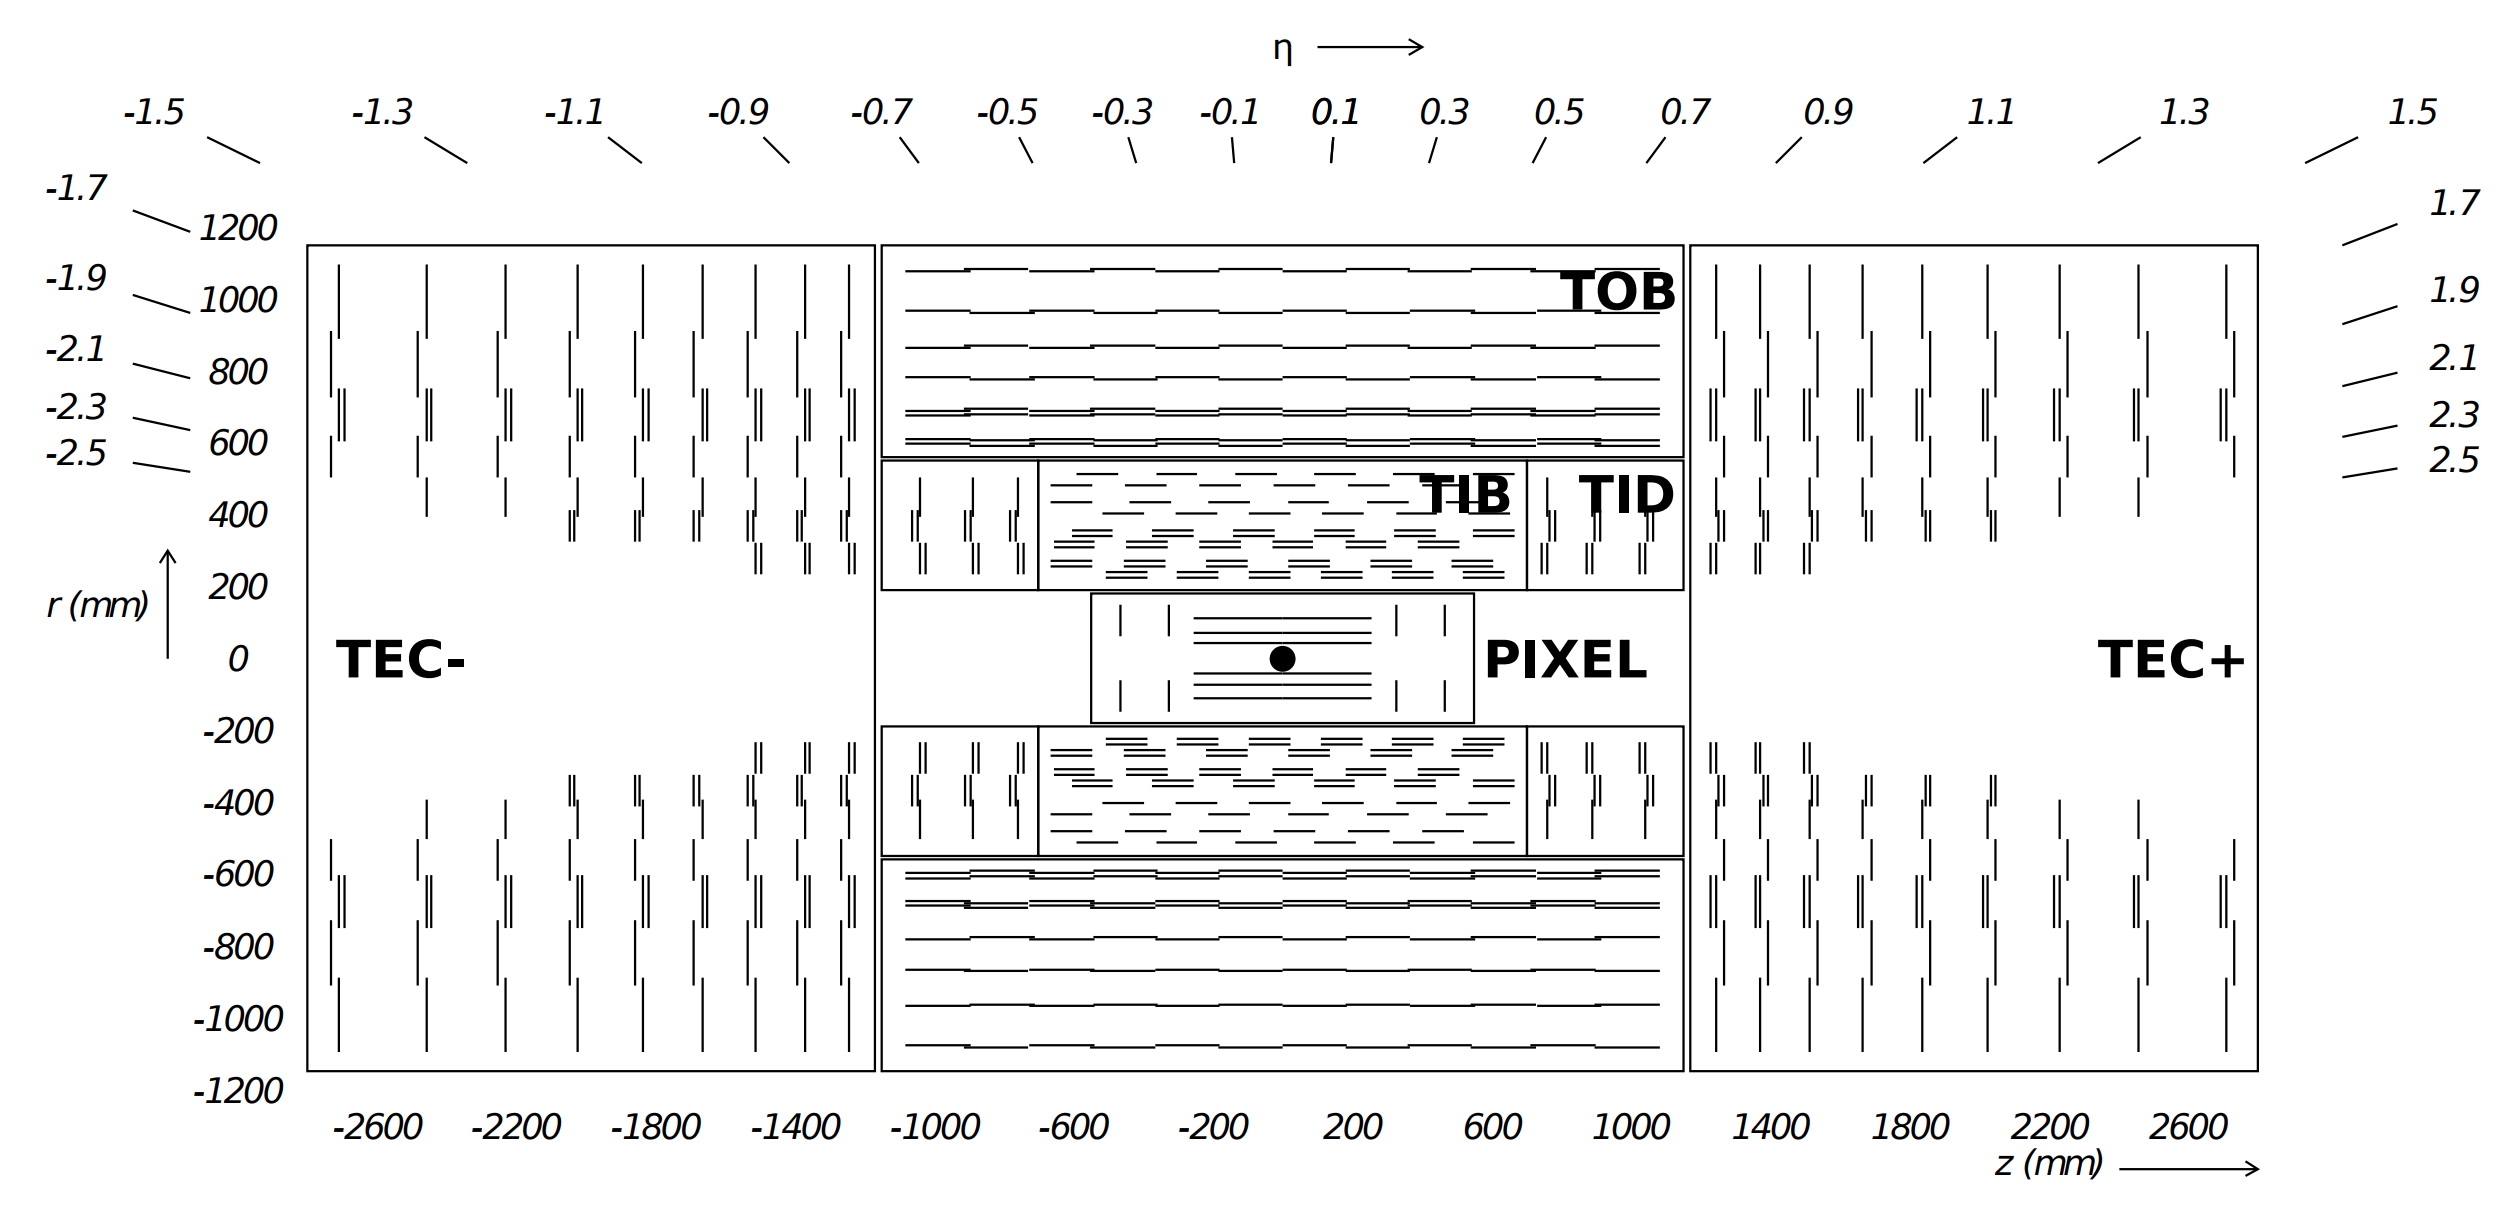
\includegraphics[width=\textwidth]{figures/LHCandCMS/trackerCrossSection.png}
  \caption{
    Cross section of the CMS tracker, viewed in the $r$-$\eta$ plane.
    At the center is the pixel detector, with the tracker inner (TIB) and
    outer barrel (TOB) instrumenting the barrel part of the detector
    at increasing distances from the beam line. The tracker inner disk (TID)
    and tracker endcap (TEC) are perpendicular to the beam pipe.
    Single lines represents a detector module, and double lines represent
    double-sided modules. Reproduced from Ref.~\cite{Chatrchyan:2009aa}.
        }
 \label{fig:trackerCrossSec}
\end{figure}

At the operating conditions of the LHC in 2016, an average of 23 proton
interactions took place per bunch crossing, producing on the order of $10^{3}$ particles
every 25\unit{ns}.
In this environment, the tracking system is crucial to determining which particles are associated
with the interaction of interest. In addition, decays displaced from the
production vertex is an important signature of heavy-flavor hadrons and $\tau$ leptons,
so knowledge of the track origins in three dimensions is crucial.
The paths of charged particles can be deduced from their discrete interactions
in the tracking system, from which the particle origin can be inferred.
Because multiple interactions in a single sensor complicate track reconstruction, the pixel and strip 
dimensions are designed to keep the particle flux per collision low.
The pixel detector barrel consists of three layers, positioned at 4.4, 7.3, and
10.2\unit{cm} from the beam line. At the inner layer,
the hit rate density is $\approx1\unit{MHz/mm}^2$, which motivates 
motivates the use of $100\times150\micron$ silicon sensors, for an occupancy
on the order of $10^{-4}$ per sensor per bunch crossing. The flux is significantly
reduced further from the beamline, so the outer parts of the tracker uses silicon
stip detectors, 10-25\unit{cm} in length and 80-180\micron in length, to reduce
the channel count and cost. In total, the silicon tracking system has over 75 million read-out channels.
The position resolution of individual sensors is $10-40\micron$,
allowing for vertex association which is accurate to $\approx10\micron$, 
and momentum resolution for muons with $\pt = 100\GeV$
and $\eta < 1.5$ is around 2\%~\cite{Chatrchyan:2014fea}.

\section{The CMS electromagnetic calorimeter}

Immediately outside the tracking system, but inside the solenoid, is the electromagnetic 
calorimeter (ECAL). It is constructed from transparent lead tungstate (\PbT) crystals, which
absorb energy of electromagnetically-interacting objects (e.g., electrons and photons) before emitting
light of wavelength $\lambda = 420$--$430\unit{nm}$, with intensity proportional to the absorbed energy.
The energy deposits of the interacting particles are obtained from
photodetectors that collect the emitted light.
Lead tungstate was chosen for properties including its high density of $8.3\unit{g/cm}^3$, which contributes
to its small radiation length---the mean distance an electron travels
in the material before loosing $1/e$ of its initial energy---of 0.89\unit{cm},
and its small Moli{\`e}xre radius (the radius at which 90\% of the electromagnetic
shower is contained on average) of 2.2\unit{cm}. These properties facilitate the 
compact design of the CMS ECAL. Because photons and electrons interact significantly
with the large physical structure of the CMS solenoid, positioning the ECAL outside
of the solenoid would degrade the energy performance and compromise the association
of tracks with ECAL energy deposits.
Consequently, a compact calorimetry system
is required to reduce the volume---and therefore the cost---of the solenoid.
In addition, the scintillation decay time of the crystals, the delay between the absorption of energy and light emission,
is such that 80\% of the light is released by an excited crystal within 25\unit{ns},
enabling the necessary fast read out. These highly favorable characteristics of {\PbT} are 
partially offset by its relatively low light output of 4.5~photons~per~MeV of deposited energy
at the operating temperature of 18\degree\unit{C}. 

\begin{figure}[htbp]
  \centering
   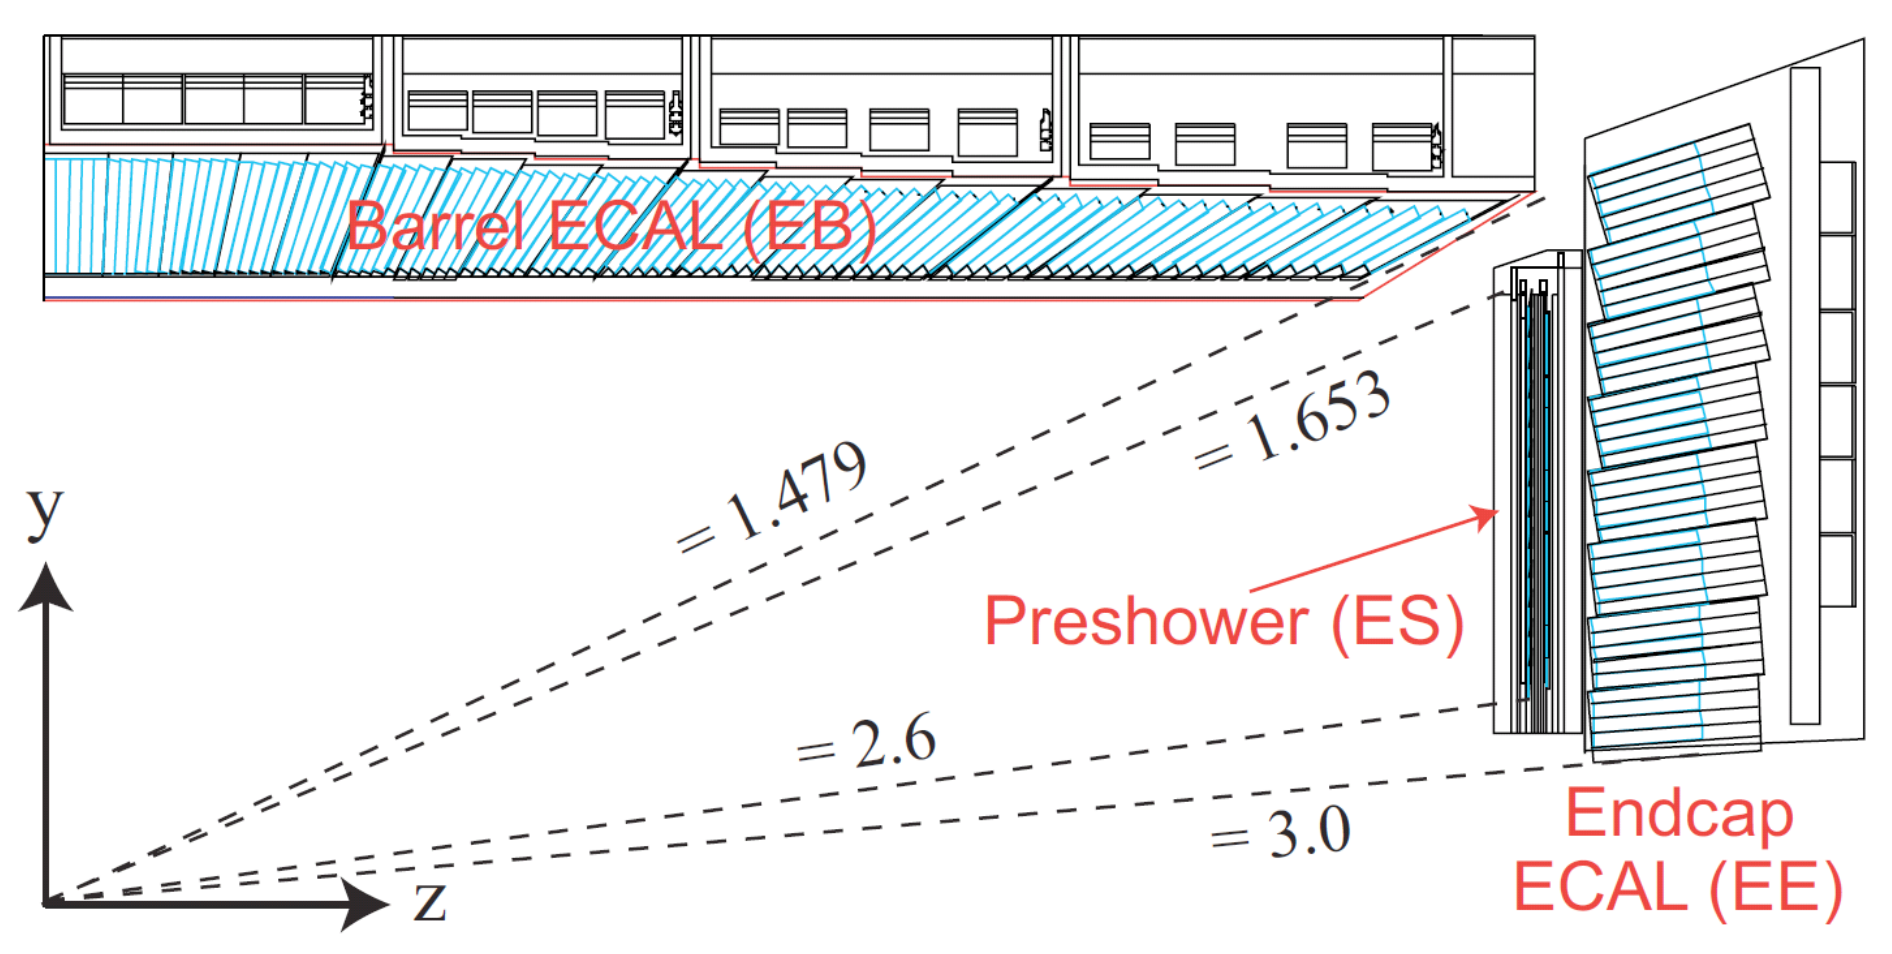
\includegraphics[width=0.6\textwidth]{figures/LHCandCMS/ecalCrossSection.png}
  \caption[An $r$-$\eta$ cross section of the CMS ECAL]{
    An $r$-$\eta$ cross section of the CMS ECAL, showing the detector components,
    crystals, and their $\eta$ coverage. Reproduced from Ref.~\ref{Benaglia:2014aqa}.
        }
 \label{fig:ecal}
\end{figure}

The ECAL system consists of 61,200 PbWO$_4$ crystals in the barrel, $\abs{\eta} < 1.444$,
and 7,324 crystals in each of two encap discs covering $1.566 < \abs{eta} < 3.0$.
The small gap in the ECAL is due to cabling and support structure for the tracking system.
The cross section of the crystals in the plane facing the interaction point is $2.2\times2.2\unit{cm}^2$,
equal to the Moli{\`e}re radius of the material. The barrel crystals are 23\unit{cm} in
length, whereas the endcap crystals are 22\unit{cm}, corresponding to 
25.8 and 24.7 radiation lengths respectively. The arrangement of the crystals is shown in Fig.~\ref{fig:ecal}.
Because of the relatively low light yield of {\PbT}, fast photodetectors with
powerful amplification capabilities, that are capable of operating in the high magnetic
field, are needed. Avalanche photodiodes instrument the barrel, while vacuum phototriodes
are used in the barrel, due to their superior radiation hardness.

The resolution of the energy measurement in the ECAL improves with energy up to 
0.5--1\TeV, at which point the percentage of the shower energy not contained in the ECAL becomes
signifiant. Below this threshold, higher energies correspond with greater light production,
and a more accurate energy measurement. The uncertainty in the energy measurement
below $\approx500\GeV$ can be parameterized as
\begin{equation}
  \left(\frac{\sigma_E}{E}\right)^2 = \left(\frac{S}{\sqrt{E/\GeVns}}\right)^2 + \left(\frac{N}{E/\GeVns}\right)^2 + C^2.
  \label{eq:resolution}
\end{equation}
Where $S$ is a stochastic term, driven by the number of scintillation photons produced,
$N$ is a noise term arising from the electronics and background radiation produced
outside the primary proton--proton interaction, and $C$ is a constant term due to
the non-uniformity of the crystal material and fabrication.
The values of $S=2.8\%$, $N=0.12$ and $C=0.30\%$ were measured in the initial 
CMS commissioning~\cite{Chatrchyan:2008aa}, 
and are illustrative of the performance during 2016 data taking.

\section{The CMS hadronic calorimeter}

Outside the ECAL, but inside the solenoid, is the hadronic calorimter (HCAL),
covering the radial space from 1.77\unit{m} to 2.95\unit{m}.
The HCAL measures energy of charged and neutral hadrons for identification
and measurement of hadronic jets. The hermetic coverage of the HCAL
up to $\abs{eta} < 5.0$ permits an extensive characterization of the 
transverse energy of hadronic particles in an event, allowing neutrinos (or weakly
interacting new physics) to be detected as an unbalance in transverse momentum.
Unlike the ECAL, the HCAL is a sampling calorimeter, that is, it is constructed
of layers of dense material to induce hadronic showers interspersed amongst 
active layers of scintillating material. 
The barrel ($\abs{\eta} < 1.3$) and endcap ($1.3 < \abs{\eta} < 3.0$) region of the HCAL are constructed from 
flat steel and brass absorber plates, 50-80\unit{mm} thick, layered between scintillating tiles.
The scintillators are segmented to cover an area in $(\eta, \phi)$ of $(0.087,0.087)$
for $\abs{\eta} < 1.6$ and $\approx(0.17,0.17)$ for $\abs{\eta} > 1.6$.
Wavelength shifting fibers adjust the wavelength to a more favorable
frequency before light is collected and measured by hybrid photodiodes.
At $\eta = 0$, the HCAL is $5.82\lambda_I$ thick, whereas it is $\approx10\lambda_I$ thick 
at $\abs{\eta} > 1.3$.
Here $\lambda_{I}$ is the nuclear interaction length, the mean free path of a hadronic particle
before undergoing an inelastic hadronic interaction.
Hadronic particles encounter about $1.1\lambda_{I}$ of material before reaching
the HCAL.

In order to measure very forward jets---which are critical for this result--a 
forward HCAL system (HF) is installed close to the beam pipe on the extreme end of the 
detector, $\pm11.15\unit{m}$ from the interaction point. 
The HF detects particles in the region $3.0 \abs{\eta} < 5.0$. Because the energy deposit
per collision in the HF is 5--10 times greater than the combined energy deposits in
the rest of the detector, the HF must be extremely radiation hard.
The active material of the HF is quartz fiber Cherenkov detectors, which 
collect radiation from particles traveling with velocity above the Cherenkov limit.
The fibers are in steel showering material. Half of the fibers extend the full length
of the detector, whereas half begin at a dept of 22\unit{cm}, which gives
sensitivity to the shower development, to distinguish between hadronic and electromagnetic
showers. The detectors are housed in a hermetic steel, concrete, 
and polyethylene shielding of 0.85\unit{m} in thickness for additional radiation
hardness. The resolution of the HF is at least a factor of two lower than the 
barrel and endcap calorimeters. Despite this, it plays an important role 
in the results presented in this thesis, which rely on forward jet reconstruction.

The layout of the HCAL, showing each subsystem discussed, as well as the small
outer part of the HCAL outside the magnet, is shown in Fig.~\ref{fig:hcal}.
As for ECAL, the energy resolution can be described by Equation~\ref{eq:resolution}.
The results obtained from pion test beams before the start of CMS
data taking are $S=115\%$ and $C = 5.5\%$. The noise term $N$ is subdominant.

\begin{figure}[htbp]
  \centering
   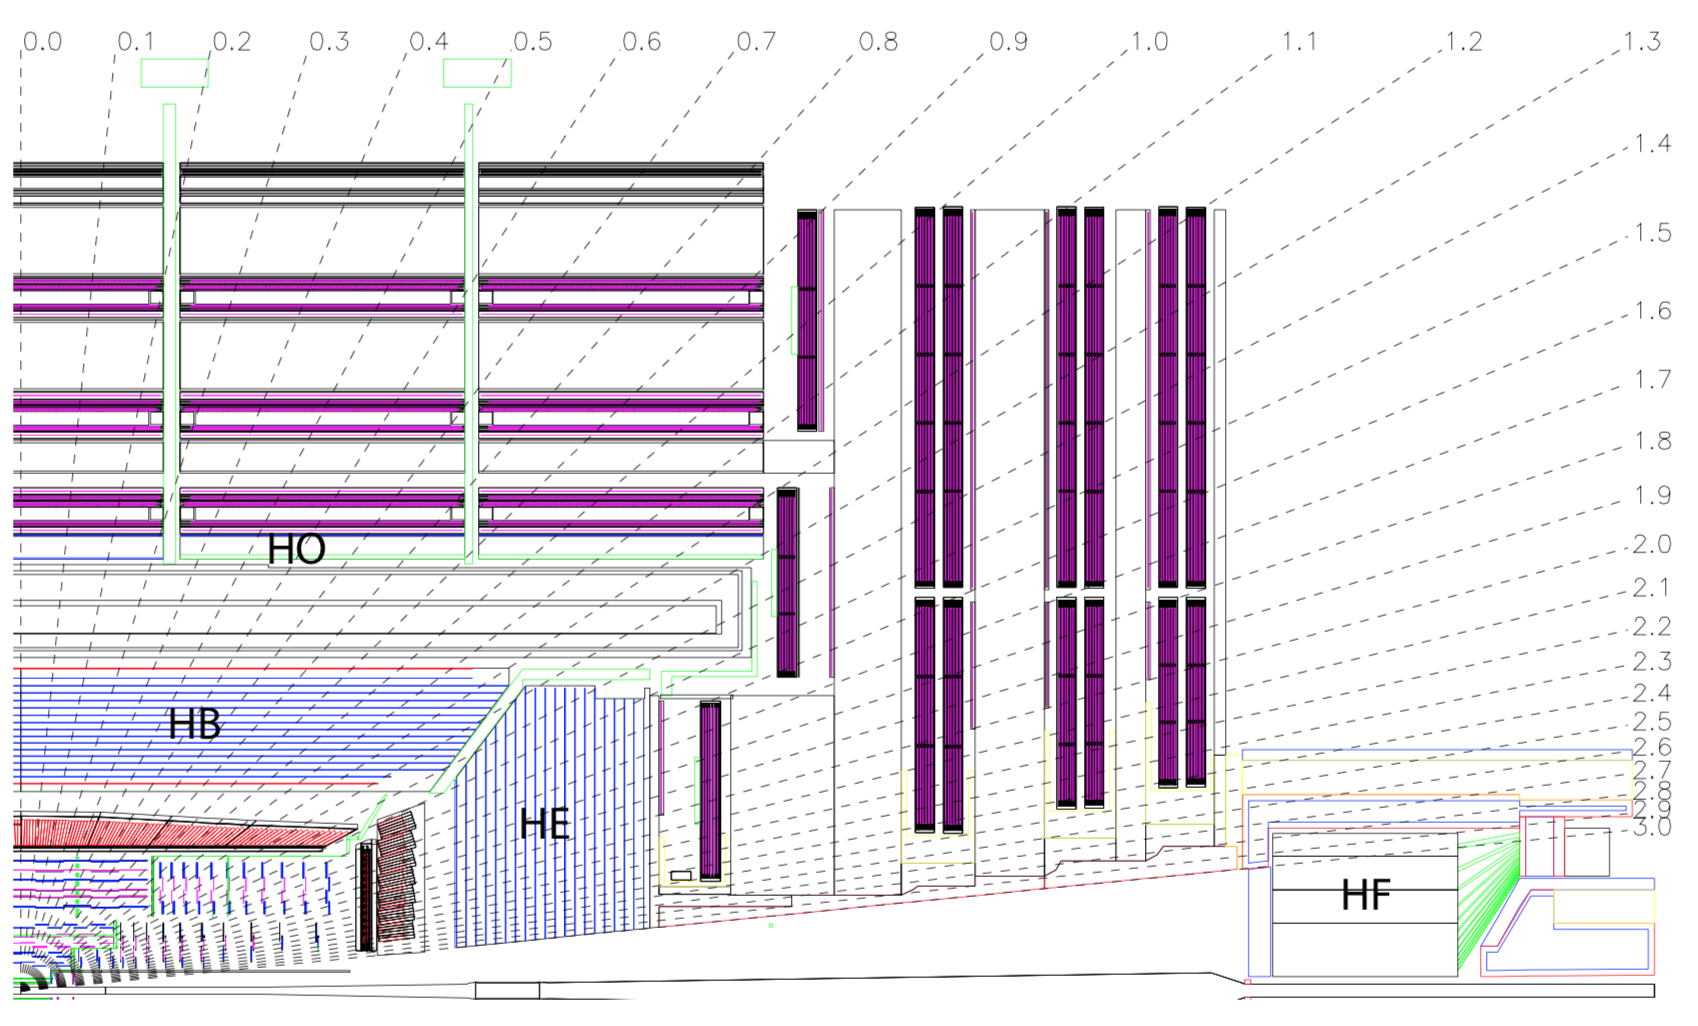
\includegraphics[width=0.6\textwidth]{figures/LHCandCMS/HCAL.png}
  \caption[An $r$-$\eta$ cross section of a quadrant of the CMS detector, showing the 
      HCAL system]{
    An $r$-$\eta$ cross section of a quadrant of the CMS detector. The components
    of the HCAL system are shown.~\cite{Chatrchyan:2012xdj}.
        }
 \label{fig:hcal}
\end{figure}

\section{The CMS muon system}

As suggested by the CMS name itself, the muon detector subsystem is essential to the
achieving the experimental goals of the CMS experiment. 
High-energy muons are produced in many heavy-object SM and BSM 
decays, and long-established detector technologies are well suited to muon detection in LHC collisions.
Muons with $v\approx c$ are nearly stable
on timescale of the traversal of the CMS detector volume. As the heavies stable lepton, 
they are less susceptible to electromagnetic radiative energy loss than electrons, and therefore
interact minimally with the calorimeter system. Detector technologies suitable for
charged-particle detection, placed outside all other detector systems, 
are therefore ideal for muon detection. 

\begin{figure}[htbp]
  \centering
   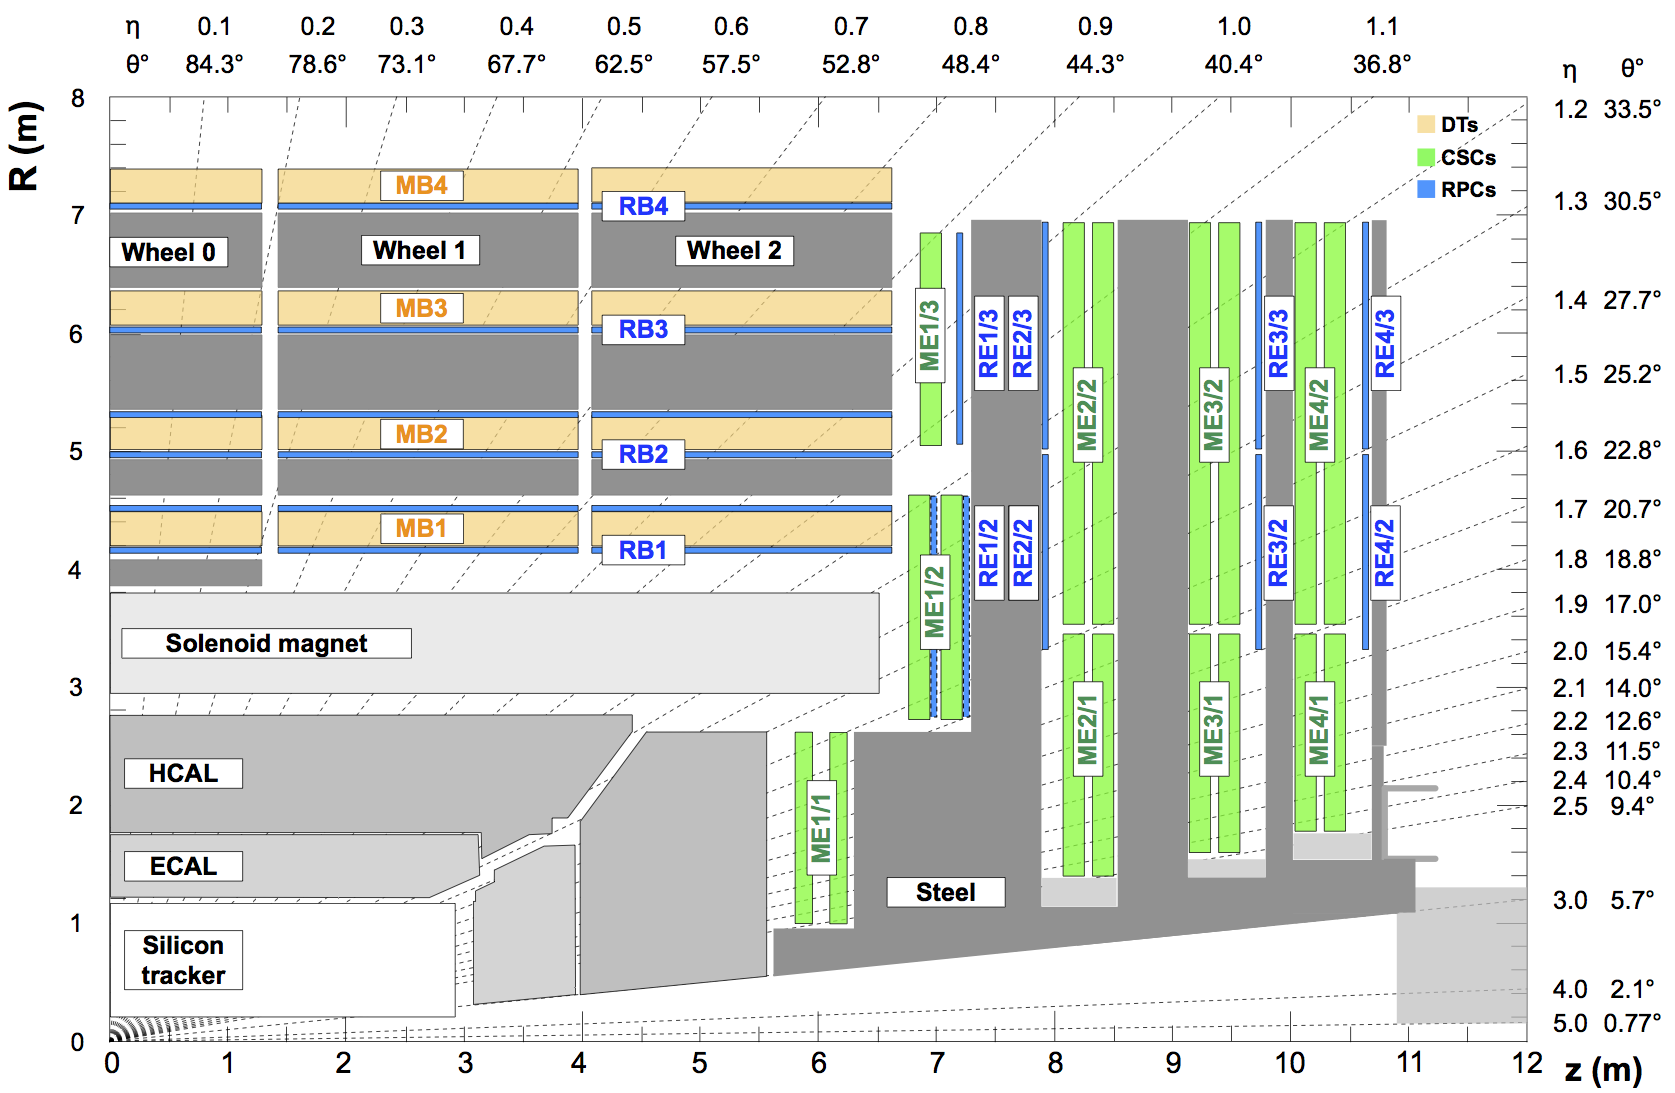
\includegraphics[width=\textwidth]{figures/LHCandCMS/MuonSystemGeometry.png}
  \caption[An $r$-$\eta$ cross section of a quadrant of the CMS detector]{
    An $r$-$\eta$ cross section of a quadrant of the CMS detector, with the interaction
    point at the bottom left corner. The locations of the detectors
    comprising the CMS muon system within the steel steel return yoke
    are shown~\cite{Chatrchyan:2012xdj}.
        }
 \label{fig:muonSystemGeo}
\end{figure}

The muon system is composed of three technologies, 
described in more detail in the following sections. 
Each operates on the principle of gas ionization. 
The detectors consist of a volume of 
gas over which an electric field is applied. Charged
particles passing through the volume ionize the gas, and the ionized gas molecules
and free electrons drift in the electric field towards read-out electronics at the 
edges of the detector volume. The track of the interacting object is inferred from
the position and timing of the measured electrons and ions.
The operating characteristics of the gas ionization detectors can be modified
for fast readout, high granularity, and 
In the CMS detector, these considerations, along with the cost of construction 
for detectors covering an area of $\approx 25,000\unit{m}^2$ and 
the effect of the radiation environment of the detector on performance, motivate
the specific design choices.

Gas ionization detectors are
sensitive to all charged particles passing through the detector. As previously discussed,
nd illustrated in Fig.~\ref{fig:muonSystemGeo}, the muon system is 
the outer layer of the CMS detector, embedded in
the steel return yoke of the magnet system. This structure, along with the inner
detector systems, serves as shielding for the muon system and ensures that the 
well over 99\% of objects reaching the muon system are muons.

\subsection{Drift tube system}

The barrel part of the muon detector, $\abs{\eta} < 1.2$,
is composed of drift tube (DT) chambers. In this region, the magnetic field
outside the return yoke is generally small (below 0.2\unit{T}), and the muon occupancy is low, justifying
the use of DT detectors. The DT system is built from individual DTs, 
rectangular aluminum tubes with a length of 2.4\unit{m} and a cross section
of $13\times42\unit{mm}^2$, shown in Fig.~\ref{fig:DTs}. At the center of each
tube is a 50-\micron-diameter gold-plated stainless-steel anode wire.
Aluminum strips are attached to the interior of the aluminum 
structure---insulated by mylar tape---to
shape the electric field to the pattern illustrated in Fig.~\ref{fig:DTs},
and an 85\% Ar 15\% CO$_2$ gas mixture is contained in the volume. 
The drift time for muons crossing a
cell at a maximum distance from the anode wire of 21\unit{mm}
is about 380\micron, which is sufficient to keep the occupancy low.
Muons passing through the gas volume ionize the gas and create an avalanche of
electrons around the very high field at the anode wire.
A time-to-digital converter reads out the electrical pulse of the electrons.
The arrival time of the signal, corrected by the drift velocity and the time
from the collisions to the trigger decision, are used to obtain the muon interaction
position. 

\begin{figure}[htbp]
  \centering
   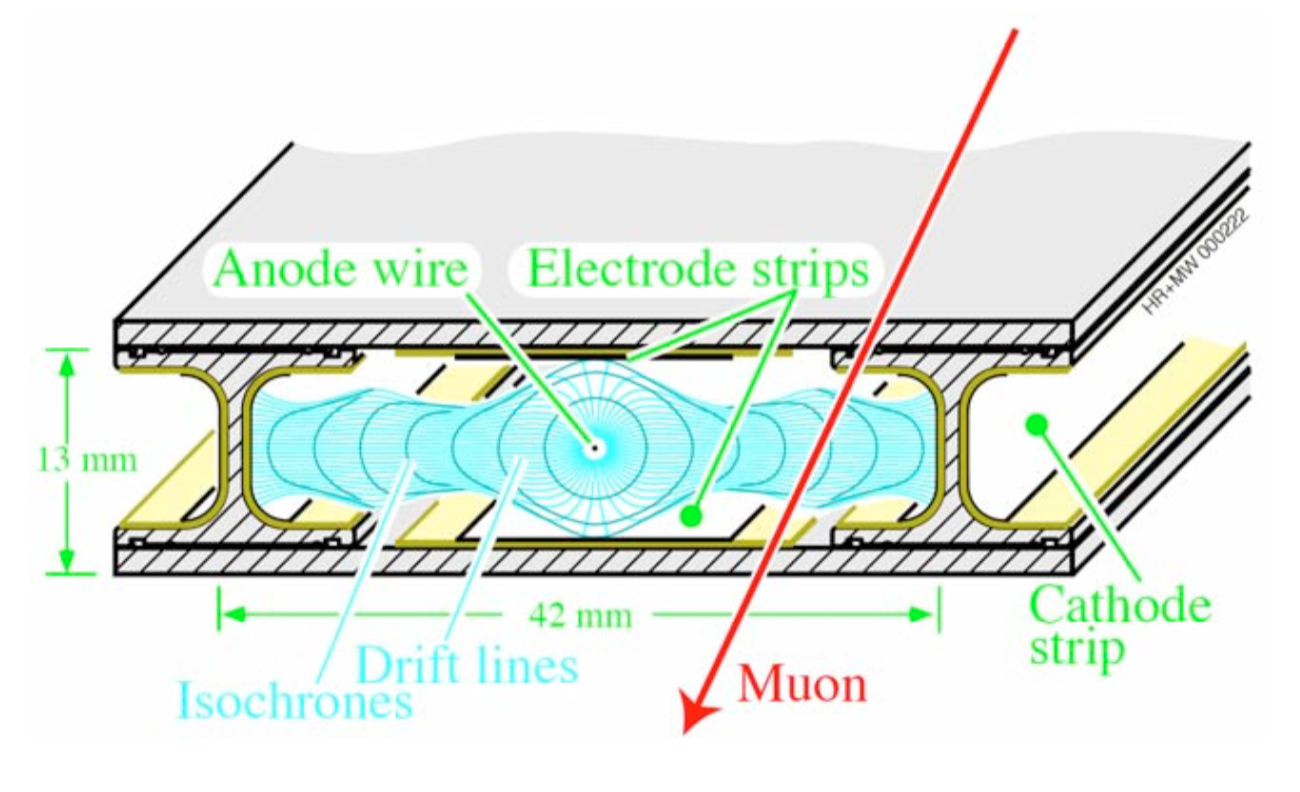
\includegraphics[width=0.6\textwidth]{figures/LHCandCMS/DriftTubeCutaway.png}
  \caption{
    Diagram of a drift tube cell, from Ref.~\cite{Chatrchyan:2008aa}. The 
    geometry of the cell and the electric field lines resulting from the 
    anode wire and electrode strips are illustrated.
        }
 \label{fig:DTs}
\end{figure}


The DT cells are assembled into superlayers (SL), composed of 
4 layers of drift cells staggered by half a cell. 
The SLs are grouped into chambers of 2 or 3 SLs which are arranged into stations
within the magnet return yoke.
The wires in the outer SLs within a chamber are parallel to beam line, providing
a measurement in the bending plane.
An additional inner SL is aligned perpendicular to the beam direction, 
for all chambers but those in the 
outermost station, to provide a measurement in the $z$ plane. 
The chambers are arranged in concentric cylinders
around the beam line, with 60 chambers each in the three inner cylinders
and 70 in the outer cylinder. In total there are $\approx172,000$ 
cells, read out as independent channels. The offset arrangement of the cells
eliminates dead spots in the efficiency, and allows a measurement of the
muon crossing time to be obtained using meantimer circuits.
The muon position resolution in the DTs is around 100\micron and the
timing resolution is within a few ns.

\subsection{Cathode strip chamber system}

Cathode strip chambers (CSC) are used in
the forward regions of the CMS detector ($0.9 < \abs{\eta} < 2.4$), 
where the prompt and background muon rates are high, and the magnetic field
is large and non-uniform. The CSC system is constructed of trapezoidal
multi-wire proportional chambers,
which subtend 20 or 30 degrees in $\phi$. The largest chambers are 3.4\unit{m}
long and up to 1.5\unit{m} wide. The chambers are divided into 6 sections---7\unit{mm} 
wide for the innermost layer of chambers and 9.5\unit{mm} for all 
others---each filled with an Ar-CO$_2$-CF$_4$ gas mixture. Aluminum cathode strips,
which span the radial direction at a constant phi, 
are milled to 6 of the panels forming the sections. The strips vary from
8.4 to 16\unit{mm}, for a constant width in $\phi$, and are separated by about 0.5\mm. 
In addition, each layer has a planes of anode wires running lengthwise, 
50\micron in diameter, separated by 2.5\unit{mm}, and slightly tilted to correct
for the deflection of the drifting electrons in magnetic field.
Muons passing through the chambers create and avalanche
of electrons in each layer, which is read out on the anode wires. In addition,
A mirror pulse is created in the cathode strips.
Together, the pulses and shapes give an excellent position measurement 
in both the $r-\phi$ and $\eta$ planes, as shown in Fig.~\ref{fig:CSC}.
Each cathode strip is read out, whereas anode strips are read out in
groups of 16. The position resolution of a CSC chamber is around
100\micron, and the timing resolution is $\approx7\unit{ns}$

\begin{figure}[htbp]
  \centering
   \includegraphics[width=0.49\textwidth]{figures/LHCandCMS/CSCdiagram.png}
   \raisebox{0.3\height}{\includegraphics[width=0.49\textwidth]{figures/LHCandCMS/CSCoperation.png}}
  \caption{
    Left: diagram of a CSC chamber. Right: principle of operation for a CSC
    layer, showing the avalanche around the anode wires and the pulse shape
    on the cathode strips, which are combined for accurate position measurement.
    Both figures are reproduced from Ref.~\cite{Chatrchyan:2008aa}
        }
 \label{fig:CSC}
\end{figure}

The CSC chambers are arranged perpendicular to the beam line,
conjoined for full coverage in $\phi$. Four stations of CSC chambers are interspersed
amongst the magnetic flux return plates in each endcap of the detector, see
Fig.~\ref{fig:CMScutaway}. The innermost station (for each endcap) is composed of 
3 rings of CSC in the radial direction, whereas other stations have two rings.
In total there are 540 CSC chambers. All but the outer ring of chambers in the 
innermost layer partially overlap the neighboring chambers, avoiding regions
of low efficiency. Members of the University of Wisconsin -- Madison 
CMS group have played a crucial role in the design and operation of the CSC
system since the inception of the CMS experiment. I contributed to the operation
of the CSC system, serving the detector-on-call for the
detector subsystem for three weeks per year from 2016 -- 2018. During these periods
I represented the CSC system in daily meetings, coordinated maintenance and 
development projects, and responded to critical issues preventing data collection
or degrading data quality.

Aging studies of the CSC chambers at the original CERN Gamma
Irradiation Facility (GIF), and at the new GIF++, have shown that the CSC system
performance is resistant to the damage incurred by the radioactive environment
of high luminosity collisions. I contributed to the on-going studies at the 
GIF++ facility by monitoring the performance of . The continued performance
of the CSC chambers after exposure to sustained radiation, comparable
to many times the luminosity already delivered to CMS,
has provided evidence that the CSC system will remain an important part
of CMS throughout the full LHC program.

\subsection{Resistive plate chamber system}

A crucial role of the muon system is to provide muon position and momentum
measurements in a sufficiently timescale
to determine if an event justifies storage offline analysis. 
This process, known as event triggering,
is described in additional detail in Section~\ref{sec:triggering}.
While the DT and CSC system provide fast readout, the background rate and
importance of associating an event with the correct bunch crossing (within
25\unit{ns}) make additional redundancy desirable.

A system of resistive plate chambers (RPC) in both the barrel and endcap
($\abs{\eta} < 1.2$ accomplishes this goal. The RPCs are double-gap chambers
constructed from a thin layer of readout strips between two electrodes held 
at high voltage, forming a volume filled predominately with C$_2$H$_2$F$_4$ gas.
The system is operated in avalanche mode, where the sum of the signals
in the two gaps created by an interacting muon is read out on strips
at the center plate. The plates are separated by 2\unit{mm}, which ensures
that the charge avalanche is observed well below the 25\unit{ns} window
needed to assign the muon to the correct bunch crossing.
There are 6 layers of RPCs in the detector barrel, interspersed among the DTs,
and 3 layers in the endcap alongside the CSCs. The readout strips in the barrel RPCs
subtend an angle of 5/16 degree. The position resolution of the RPCs, about 1\cm,
is below the DT and CSC systems, but the system provides an independent position
and timing measurement. 

\section{Event triggering and data acquisition}

Despite significant zero-suppression and data compression, the
read out from the millions of channels in the CMS detector for
a typical proton--proton collision of interest requires around
1\unit{MB} of storage.
Transmitting this quantity of information 
at the collision rate of 40\unit{MHz} delivered by the LHC to the CMS detector 
exceeds the threshold of practical technological capabilities. Furthermore,
the event rate of rare standard model processes and theorized BSM interactions
is many orders of magnitude below this rate. 
Therefore, it is neither feasible 
nor desirable to store every collision.

The CMS trigger system uses a two-tiered approach to selecting events of 
interest---typically characterized by having one or more objects
at high missing transverse momentum---and rejecting more common proton 
interactions, such as elastic electromagnetic scattering.
The Level 1 (L1) trigger is a custom-designed hardware system,
primarily built from programmable electronics, that
is designed to reduce the rate of collisions to below 100\unit{kHz}
in a latency of about 4\mus. The L1 trigger decision,
known as an ``L1 accept`` when an event is stored,
uses coarsely segmented
information from the muon and calorimeter systems.
Information in the inner tracker is not used at L1, due to the read-out
latency of the system. 

The L1 trigger system initially handles the calorimeter and muon system
information independently. For the calorimeter information, the ECAL crystals
are grouped into towers of 25 crystals, to match the HCAL granularity
in $\eta$ and $\phi$ space and to reduce granularity. Energy deposits in
the ECAL and HCAL are used to build primitive objects, e.g., 
the energy and shape of ECAL deposits
contribute to photon and electron candidates while HCAL information
suggests clusters of hadronic particles produces in the event.
The particle candidates are sorted by $\pt$, and the total energy deposit
in the event is computed, before forwarding the event information to
the global trigger for an event-wide decision.

The muon trigger system builds track candidates by matching hit
patterns in the CSC, the DT, and the RPC subsystems. Track finders
specific to the barrel region ($\abs{\eta} < 0.9$), the endcap region
($0.9 < \abs{\eta} < 1.2$), and the CSC-DT overlap region ($1.2 < \abs{\eta} < 2.4$),
combine the track segments from individual detectors to form muon
candidates. The candidates built by each track finder are combined
and disambiguated by the global muon trigger, which sorts the 
candidate objects by \pt before forwarding them to the global trigger.

The global trigger uses the sorted candidate and event information from
the muon and calorimeter triggers to test for
tests for the physics objects and object combinations,
based on kinematic and quality criteria, before accepting or rejecting
the event. The set of conditions by which events are evaluated
are organized into ``trigger paths,'' which act to sorting the 
dataset and the procedure by which it is evaluated. For paths 
with very high rate, e.g., signal lepton triggers with lower \pt
thresholds, a trigger path may be ``prescaled.'' This process 
reduces the event rate by rejecting an unbiased subset of the events
otherwise satisfying the acceptance criteria. Prescaled trigger paths
are important for validating the efficiency and performance of other
trigger paths.

Data collected by the detector system is continually read and stored into
40-MHz pipelined buffers while waiting for a trigger decision to determine
if the data should be overwritten by the continual stream of new data,
or pushed to the next stage of the data acquisition system for storage.
The $4\,\mu s$ window for the trigger decision is set by the storage capacity
of the most limited buffer system, associated with the silicon tracker.
If the L1 trigger determines an event should be read for further analysis,
the data are forwarded over a high-bandwidth network system to a 
processing farm for further analysis. The read-out bandwidth limits the 
rate of accepted events at L1 to about 100\unit{kHz}. In some cases, it is
necessary to explicitly enforce this condition, accomplished through
the trigger throttling system. The trigger throttling system prevents event
read out in cases where a subsystem data buffer is near capacity,
or when event triggering in quick succession would lead to excessive rate. For example,
the trigger throttling system prevents event read out for three successive
bunch crossing after a triggered event. This reduction in event readout,
referred to as deadtime, is generally unbiased and kept below 1\%. However,
for this analysis, a systematic loss of events due to mistimed
trigger signals lead to an inefficiency in collection of events of interest. This
effect is discussed in detail in Chapter~\ref{ch:analysis}.

Events accepted by the L1 trigger undergo an additional filtering 
by the high level trigger (HLT) before they are stored to tape for offline analysis.
The HLT is a software-based system running on a commercial processing farm that
has access to the full event information from all detector systems. In principle,
the HLT can implement the same reconstruction algorithms described in Chapter~\ref{ch:reconstruction},
but the time constraints for the decision and the limited size of the compute farm
make this impractical. Instead, the HLT implements similar algorithms with
optimizations and simplifications designed to reach an event acceptance or rejection
decision in less than 200\mus. As with the L1 trigger, the event evaluation is
divided into trigger paths. Operations are performed per trigger path such that
uninteresting events are rejected as soon as possible, with computationally
expensive operations such as track building only performed at the final stages.
The high cost of large-scale data storage, especially in a way that allows quick access 
for processing at sites throughout the world, is an increasing concern for the
LHC experimental program. In addition to ensuring manageable read-out rates,
efficient filtering by the HLT is an important to addressing this storage issue.

\label{sec:triggering}
\section{Luminosity measurement}

The luminosity delivered by the LHC to the CMS interaction point is a critical
input parameter to any cross section measurement and many LHC searches, as it 
is needed to established the expected background contribution from processes
described by MC simulation and to convert an observed event rate to an measured
cross section. Luminosity is defined purely in terms of the parameters of the 
LHC, as given by Equation~\ref{eq:lumi}. However, because the conditions of the LHC beams
are not constant throughout a data collection period (e.g., the number of protons
in the colliding bunches decreases continually during an LHC fill),
the instantaneous luminosity must be continually monitored. Establishing
the luminosity in terms of the parameters in Equation~\ref{eq:lumi} while the LHC
is delivering collisions is unfavorable
because measurements of the beam parameters, such as the beam widths,
cannot be made to high precision without interfering with the beam conditions.
Instead, the luminosity can be monitored by exploiting the relationship between
luminosity and detector occupancy, which is linear for the primary the current
LHC operating conditions and the detector systems considered for the 
measurement~\cite{CMS-PAS-LUM-13-001}.
Therefore, the relationship between the observed occupancy 
rate and the luminosity can be expressed as
\begin{equation}
  R = \sigma_{vis}\mathcal{L}\,,
  \label{eq:lumiRate}
\end{equation}
where the proportionality constant $\sigma_{vis}$ is known as the visible cross
section seen by the detector system. By establishing $\mathcal{L}$ and $\sigma_{vis}$
in conditions where the parameters of Equation~\ref{eq:lumi} are known, further monitoring
of the luminosity can be achieved purely via a measurements of the $R$.

The reference luminosity measurement is accomplished in dedicated LHC run periods using 
a technique established by Simon Van der Meer at the CERN intersecting storage
rings in 1968~\cite{vanderMeer:296752}. During these periods, the $x$ and $y$ positions of the LHC beams are
scanned from their nominal head-on alignment used during collision by controlled distances.
Because the number of colliding protons depends on the beam overlap,
the occupancy rate in the detector can be used to establish the Gaussian profiles of 
the beams. Combined with the rate at nominal collision alignment and the beam intensity,
this procedure, referred to as a Van der Meer scan, establishes the relationship of 
Equation~\ref{eq:lumiRate}.
The CMS experiment monitors the luminosity by measuring the occupancy
in the pixel detector, the DT system, and the HF. In addition, two detector
systems dedicated to the luminosity measurement are used, the fast beam conditions monitor 
and the pixel luminosity telescope. A separate $R_i$ and $\sigma_{vis}$ is obtained for
each monitoring system, so the consistency of the independent measurements can be used
for validation. 
The consistency of different approaches to monitoring the luminosity,
along with uncertainties in establishing the beam parameters in the Van der Meer scan,
contribute to the systematic uncertainty of the luminosity measurement. For the 2016
dataset, the luminosity is established with a systematic uncertainty of 2.5\%~\cite{CMS-PAS-LUM-17-001}.
Calibrated values of the luminosity are established
In 2016, the LHC delivered $41.0\fbinv$ of {\pp} collisions to the CMS interaction point.

\section{CMS Data quality}

The CMS detector collects data from collisions delivered by the LHC to the CMS interaction point
with all components of the CMS detector active, configured, and synchronized. In some cases,
issues with a subsystem status or configuration prevent data collection. Reasons for data loss include, e.g., 
trigger throttling (discussed in the previous section), or problems with
high or low voltage power supplies that require manual intervention to recover detector operation.
In 2016, the CMS experiment collected 92\% of the data delivered by the LHC. 

Collected data
are evaluated by experts from each subsystem to assess the detector performance, because 
problems that did not prevent data collection can still compromise its utility for physics analysis.
For example, collected data with severe localized inefficiencies that prevent 
object reconstruction in a kinematic region and bias results in a complex way are excluded from 
the data set used for analysis.
This analysis uses only data certified by the CMS
experiment for physics analysis, which corresponds to 95\% of the collected data.

\begin{figure}[htbp]
  \centering
   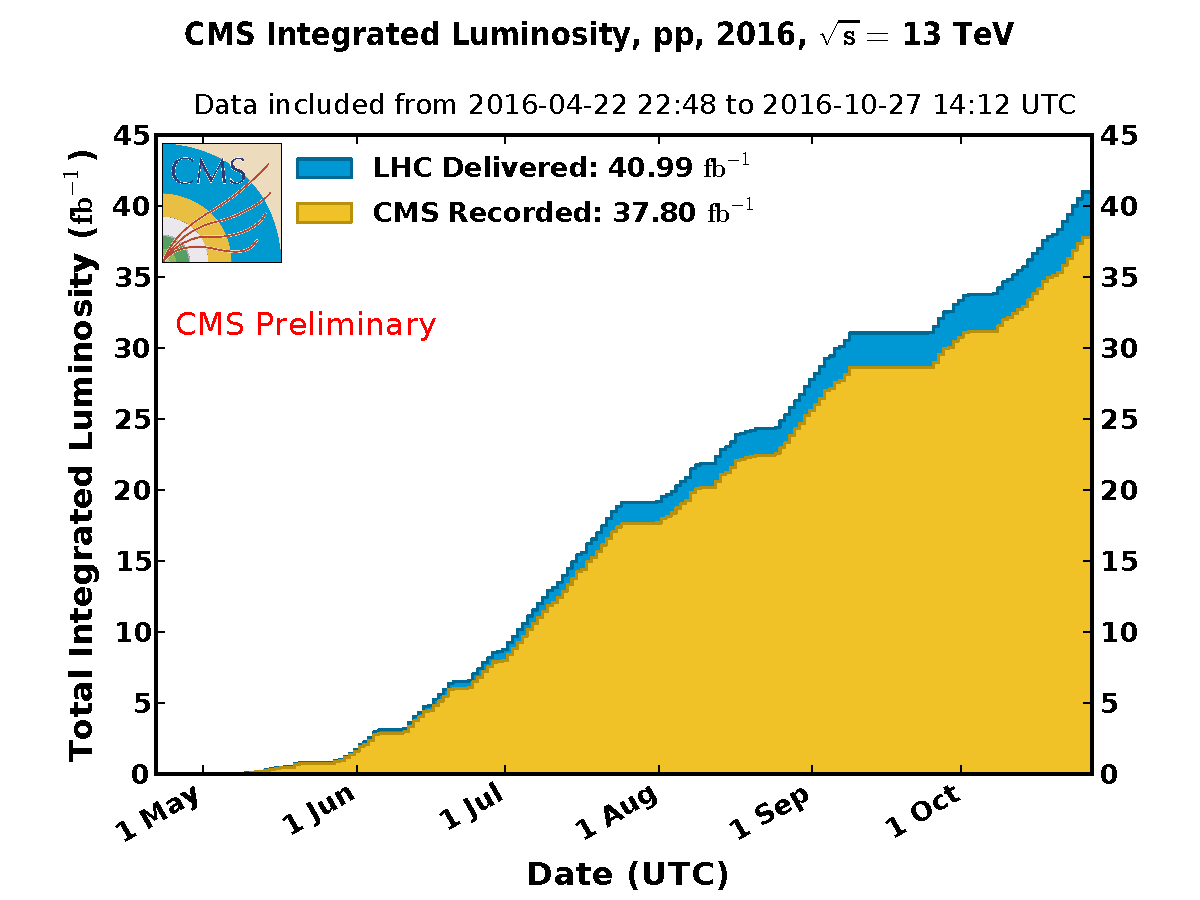
\includegraphics[width=0.6\textwidth]{figures/LHCandCMS/int_lumi_per_day_cumulative_pp_2016.pdf}
  \caption{
    The accumulated luminosity of the data delivered to the CMS interaction point, 
    collected by the CMS experiment, and approved for physics analysis by detector
    experts, are shown. Reproduced from Ref.~\cite{lumiTwiki}
        }
 \label{fig:lumi}
\end{figure}

I represented the CSC subsystem as the primary data certification expert during 
the collection of data used in this thesis.
Because of the large redundancy of the CSC chamber layout, the CSC system approved over 99\% of the
collected data for physics analysis. A water leak at the end of 2016 in the CSC cooling system 
necessitating a large-scale shutdown of the inner 
CSC chambers was the major source of data loss, however, this primarily effected \pp collisions
at 5\TeV, which are not used in this thesis. The source of the problem was identified during
the early-2017 LHC shutdown, and repaired by reinforcing the connections of the copper pipe cooling system.
